In dem folgenden Kapitel sollen die Ergebnisse der unterschiedlichen Implementierungen ausgewertet und analysiert werden. Dafür werden einige ausgewählte Kriterien anhand der Implementierungen und weiteren Quellen bestimmt und anschließend analysiert.

\section{Performance und Entwicklung}
Ein wichtiger Faktor bei der Entwicklung einer Applikation ist die Applikations-Performance. Da diese die Erfahrung bei der Benutzung beeinflusst, sollten Apps möglichst performant laufen, um die Ressourcen des Gerätes zu schonen und eine flüssige UI zu garantieren. Außerdem benötigen Entwickler einen einfachen und zeitsparenden Ablauf für typische Entwicklungsoperationen, wie etwa das anfängliche Kompilieren, oder das Laden von Änderungen. Auch die Möglichkeiten des Debuggens und Testens spielen bei der Entwicklung eine Rolle. Diese Faktoren sollen im Folgenden analysiert werden.

\subsubsection{Performance}

\begin{table}[ht]
\centering
\caption{Performancemessung der verschiedenen Applikationen}
\begin{tabular}{ |p{3.5cm}||>{\raggedleft\arraybackslash}p{2.5cm}|
>{\raggedleft\arraybackslash}p{2.5cm}|
>{\raggedleft\arraybackslash}p{3.5cm}|
>{\raggedleft\arraybackslash}p{2.5cm}|}
 \hline
 \multicolumn{1}{|>{\centering\arraybackslash}p{3.5cm}||}{} &
 \multicolumn{1}{>{\centering\arraybackslash}p{2.5cm}|}{native\break Applikation}  &
 \multicolumn{1}{>{\centering\arraybackslash}p{2.5cm}|}{hybride\newline Applikation} &
 \multicolumn{1}{>{\centering\arraybackslash}p{3.5cm}|}{cross-kompilierte Applikation} &
 \multicolumn{1}{>{\centering\arraybackslash}p{2.5cm}|}{gemischte Applikation} \\
 \hline
Durchschnittliche CPU- Auslastung & 0,9 \%    & 1,8 \%    & 1,96 \%   & 2,54 \%    \\ \hline
Maximale\newline CPU-Auslastung         & 3,6 \%    & 7,4 \%    & 6,4 \%    & 9,8 \%     \\ \hline
Durchschnittliche RAM-Auslastung & 86,74 MB  & 107,68 MB & 150,68 MB & 215,38 MB \\ \hline
Maximale\newline RAM-Auslastung         & 100,64 MB & 117,06 MB & 175,46 MB & 238,00 MB  \\ \hline
App-Größe                        & 5,2 MB    & 4,4 MB    & 7,2 MB    & 7,4 MB     \\ \hline
Maximale Startzeit               & 263 ms    & 486 ms    & 452 ms    & 532 ms     \\ \hline
Durchschnittliche Renderzeit     & 9,04 ms   & 21,88 ms  & 5,12 ms   & 8,68 ms    \\ \hline
\end{tabular}
\label{tab:evaluations_performance}
\end{table}
\newpage
In Tabelle \ref{tab:evaluations_performance} sind die Ergebnisse der Performance-Messungen zu sehen, die an den in Kapitel \ref{cha:4_Entwicklung} beschriebenen Implementierungen durchgeführt wurden. Dabei wurde die durchschnittliche und maximale Auslastung der CPU und des RAMs, sowie die App-Größe, maximale Startzeit der Applikation und die durchschnittliche Renderzeit gemessen. 
Die Renderzeit entspricht dabei der Zeit, die benötigt wird, bis eine Änderung der Benutzeroberfläche, angezeigt werden kann.

Die Messungen wurden mit dem Programm Apptim\footnote{\url{https://www.apptim.com/}} durchgeführt. Dieses zeichnet die Performance von Applikationen während der Ausführung auf einem verbundenen Gerät auf. Die Tests wurden mit einem Google Pixel 5 durchgeführt, welches mit Android 12 beziehungsweise API Level 31 läuft. Es hat dabei 8GB DDR4-RAM und eine 8-Kern-CPU, die mit durchschnittlich 1,9 GHz getaktet ist.
Der Test wurde dabei für jede Implementierung fünf Mal wiederholt und am Ende aus den Ergebnissen ein Durchschnittswert gebildet.
Die Apps wurden nach jeder Nutzung zurückgesetzt und alle anderen Applikationen wurden während der Tests beendet.
Zusätzlich wurde jeweils die Release-Version der Applikationen installiert, so dass die Performance gemessen wird, die auch ein Nutzer tatsächlich erleben würde.

Hierbei ist erkennbar, dass die native Implementierung insgesamt die performanteste ist und dabei in etwa die Hälfte der Auslastung erreicht, die die cross-kompilierte Applikation benötigt.
Dahingegen hat die gemischte App im Vergleich die höchste Auslastung und benötigt die längste Startzeit.
Nach Programmiersprachen betrachtet, haben die mit Dart programmierten Flutter Applikationen die geringste Renderzeit, während sie jedoch mehr RAM benötigen als die mit Kotlin implementierten Applikationen.
Die Implementierungen mit einem Web-Container, also die Hybride und Gemischte, verschlechtern sich im Vergleich zu den anderen beiden Implementierungen in der Performance deutlich. Daraus lässt sich schließen, dass ein Web-Container eine Performanceverschlechterung verursacht. So ist etwa die hybride Applikation in den Messwerten ähnlich zu der cross-kompilierten Applikation, obwohl sie lediglich einen Web-Container ausführt und anzeigt, während die Flutter App hingegen die komplette Benutzeroberfläche und Kommunikation mit dem Server ausführt. Dies ist auch in der deutlich geringeren App-Größe der hybriden-Applikation zu erkennen.  

Die geringere Renderzeit der Flutter Applikationen ist insofern unerwartet, da Flutter die Applikation in nativen Code übersetzt und somit eine ähnliche bis schlechtere Leistung zu erwarten wäre. Jedoch nutzt Flutter für die UI keinen nativen Code, sondern eine eigene Grafikbibliothek namens Skia\footnote{\url{https://skia.org/}}. Mit Hilfe von Skia sind Flutter Apps von der Renderpipeline des nativen Systems unabhängig und erreichen dadurch eine kürzere Renderzeit \cite{Thiele_2018}. Dabei werden bei Flutter die einzelnen Elemente der Benutzeroberfläche auf eine Art Leinwand gemalt. Die Oberfläche wirkt dabei dennoch nativ für die Plattformen Android und iOS, da je nach Plattform unterschiedliche Designgrundlagen verwendet werden, um die UI zu erstellen\cite{jose_flutter}. Des Weiteren nutzt Flutter, wie in Kapitel \ref{cha:4_3_1} erklärt, ein auf dem Widget definierten State, um Benutzeroberflächen nur partiell neu bauen zu müssen.

Biørn-Hansen et al\cite{BirnHansen.2020} sagen in ihrer Auswertung, dass sie eine deutliche Verschlechterung der Performance von Flutter bei der Nutzung einer Datenbank feststellen konnten. Deshalb wurde sowohl die Flutter App als auch die native Android App jeweils mit und ohne eine Datenbank gemessen und der Unterschied zwischen den zwei Messungen berechnet. Das Ergebnis ist dabei in Tabelle \ref{tab:evaluations_performance_Overhead_database} zu sehen.

\begin{table}[ht]
\centering
\caption{Unterschied bei Implementierung mit zusätzlicher Datenbankimplementierung}
\begin{tabular}{ |p{7cm}||>{\raggedleft\arraybackslash}p{3cm}|>{\raggedleft\arraybackslash}p{3cm}|}
 \hline
  \multicolumn{1}{|>{\centering\arraybackslash}p{7cm}||}{} & \multicolumn{1}{>{\centering\arraybackslash}p{3cm}|}{Flutter} &  \multicolumn{1}{>{\centering\arraybackslash}p{3cm}|}{Kotlin-Nativ} \\
 \hline
 Durchschnittliche CPU-Auslastung       &  0,44 \%&   0,26 \%\\
  \hline
 Maximale CPU-Auslastung  & 2,2 \%& 2,6 \%\\
  \hline
 Durchschnittliche RAM-Auslastung & 5,64 MB& 18,04 MB\\
  \hline
 Maximale RAM-Auslastung & 4,98 MB& 39,64 MB\\
  \hline
 App-Größe & 0,1 MB& 0,1 MB\\
  \hline
 Maximale Startzeit & 221 ms& 162 ms\\
 \hline
 Durchschnittliche Renderzeit &0,82 ms& 4,68 ms\\
 \hline
\end{tabular}
\label{tab:evaluations_performance_Overhead_database}
\end{table}

Die Ergebnisse zeigen einen Anstieg der RAM Auslastung, der bei der nativen Implementierung etwa drei Mal so hoch ist, wie bei der cross-kompilierten Flutter Implementierung. Dafür ist die Startzeit und durchschnittliche CPU-Auslastung bei der Flutter Implementierung stärker angestiegen als bei der Nativen. Dennoch kann anhand der Messungen kein deutlicher Unterschied für die Nutzung einer Datenbank zwischen einer Flutter Anwendungen und nativer Applikation festgestellt werden.

Bezüglich der Performance kann zusammenfassend festgestellt werden, dass die native Implementierung am besten ist. Die cross-kompilierte Implementierung mit Flutter kann dennoch durch die schnelle Renderzeit überzeugen und ist für den Nutzer nicht spürbar langsamer, da die Unterschiede im Millisekunden- beziehungsweise im einstelligen Prozentebereich liegen. Die Nutzung einer WebView, wie sie die gemischte und die hybride App benutzen, hat sich außerdem als negativer Faktor für die Performance herausgestellt.
Insgesamt lässt dies den Schluss zu, dass bei einer hohen Dringlichkeit der Performance eine native Entwicklung ratsam ist, jedoch eine cross-kompilierte Flutter-Implementierung ebenfalls möglich ist.

\subsubsection{Dauer typischer Entwicklungsoperationen}
Die Dauer der typischen Entwicklungsoperationen, wie beispielsweise die Kompilierzeit, bestimmt wie einfach Applikationen entwickelt werden können. Oft müssen bei der Entwicklung von Oberflächen kleinere Anpassungen vorgenommen und anschließend überprüft werden, ob diese den gewünschten Effekt hatten. Deshalb sind vor allem kurze Ladezeiten von Änderungen besonders wichtig.

Zwar hängt die genaue Dauer stets von der zur Verfügung stehenden Hardware, sowie der Größe des Projektes ab, die hier gemessenen Werte können dennoch gut für einen Vergleich verwendet werden. 
Für diese Arbeit wurden die Tests wiederum fünf Mal wiederholt und am Ende ein Durchschnitt gebildet. Als Hardware wurde ein PC mit 32GB RAM und einer Ryzen 5 2600 CPU genutzt. 
Die gemessenen Parameter sind dabei die Dauer des erstmaligen Kompilierens, die Dauer eines Neubaus auf Basis eines bestehenden Cache, die Dauer bis Layout- beziehungsweise Anwendungslogik-Änderungen geladen wurden. 
Die Tests für diese Werte wurden im Debug-Modus durchgeführt. Dieser ist der typische Modus während der Entwicklung, vor allem, da er das Debuggen der Anwendung ermöglicht. Zusätzlich zu den Messungen im Debug-Modus wurde außerdem noch die Kompilierzeit im Release Modus aufgezeichnet, um zu bestimmen, wie lange es dauert eine Version zur Veröffentlichung zu bauen. Die Ergebnisse der Messungen sind in Tabelle \ref{tab:evaluations_build_time} zu sehen.

\begin{table}
\centering
\caption{Dauer typischer Entwicklungsoperationen in Sekunden}
\begin{tabular}{ |p{3.5cm}||>{\raggedleft\arraybackslash}p{2.5cm}|
>{\raggedleft\arraybackslash}p{2.5cm}|
>{\raggedleft\arraybackslash}p{3.5cm}|
>{\raggedleft\arraybackslash}p{2.5cm}| }
 \hline
 \multicolumn{1}{|>{\centering\arraybackslash}p{3.5cm}||}{} &
 \multicolumn{1}{>{\centering\arraybackslash}p{2.5cm}|}{native\break Applikation}  &
 \multicolumn{1}{>{\centering\arraybackslash}p{2.5cm}|}{hybride\newline Applikation} &
 \multicolumn{1}{>{\centering\arraybackslash}p{3.5cm}|}{cross-kompilierte Applikation} &
 \multicolumn{1}{>{\centering\arraybackslash}p{2.5cm}|}{gemischte Applikation} \\
 \hline
Build Zeit Release           & 40,92 & 22,42 & 54,22 & 59,20 \\ \hline
Build Zeit Debug             & 20,20 & 20,19 & 28,76 & 33,78 \\ \hline
Erneuter Build mit Cache     & 3,36  & 3,21  & 8,36  & 8,80  \\ \hline
Neuladen nach Layoutänderung & 2,59  & 2,64  & 0,60  & 0,59  \\ \hline
Neuladen nach Logikänderung  & 3,183 & 2,635 & 0,622 & 0,626 \\ \hline
\end{tabular}
\label{tab:evaluations_build_time}
\end{table}

Bei der Analyse der Daten fällt auf, dass die zum Bauen benötigt Zeit bei den Flutter Applikationen im Vergleich zu den mit Kotlin implementierten Ansätzen höher ist. 
Auch bei erneuten Bauen, mit vorhandenem Build-Cache, sind die Kotlin-Versionen etwa doppelt so schnell wie die Flutter Implementierungen.
Mit Ausnahme des hybriden Ansatzes, braucht die Erstellung der Release-Version etwa doppelt so lang wie die Debug-Version. 
Bei der hybriden Version ist hier kein großer Unterschied, was auf die geringe Größe der Codebasis zurückzuführen ist.

Ein großer Unterschied ist bei der Neuladezeit nach einer Änderung im Quellcode festzustellen. Dieser entsteht, da Flutter dank des so genannten HotReload Feature deutlich schnelleres neu laden ermöglicht. Daher benötigen die Flutter Applikationen gerade einmal 1/5 der Zeit der Kotlin Applikationen. Dazu kommt, dass beim Neuladen mit Kotlin, die Applikation auf dem Startbildschirm startet, während Flutter lediglich die Änderungen in die aktuelle Seite lädt und diese neu rendert. Dadurch muss nicht wieder zur derzeitig entwickelten Ansicht zurückgekehrt werden. Wird beispielsweise die Farbe eines Textes im Fluttercode geändert, dann kann diese Änderung innerhalb von 600ms angezeigt werden. Dadurch kann ein Entwickler nicht nur Zeit einsparen, sondern sich zusätzlich besser auf die eigentliche Entwicklung der Benutzeroberfläche konzentrieren.

Die schnelle Ladezeiten kann Flutter aufgrund seiner zugrunde liegenden Architektur erreichen. Zwar erzeugt Flutter im Release-Modus eine cross-kompilierte Anwendung. Jedoch wird im Debug-Modus hingegen eine interpretierte Anwendung erzeugt \cite{flutter_debug_dart}. Dazu wird der Dart Code in diesem Modus nicht im Vornherein kompiliert, sondern erst wenn der entsprechende Code ausgeführt wird. Folglich müssen die Änderungen nur an die entsprechende Stelle geladen werden und die aktuell angezeigte Seite neu gebaut werden. Dadurch sinkt jedoch die Performance der Applikation, da wie bei anderen interpretierten Applikationen, der Code vor jeder Ausführung compiliert werden muss. Dies ist im Debug Modus jedoch nicht entscheidend, da hier der Fokus auf dem schnellen Entwickeln liegt. Flutter bietet außerdem noch einen dritten Modus an, in dem eine Applikation auf einem Gerät installiert werden kann, der sogenannte Profile-Modus \footnote{\url{https://docs.flutter.dev/testing/build-modes\#profile}} \cite{flutter_debug_dart}. 
Dieser wird benötigt, um eine Überprüfung der korrekten Funktionalität der cross-kompilierten Version zu ermöglichen, während immer noch die Möglichkeit besteht den Code zu debuggen. Daher wird in diesem Modus die App bereits im vornherein kompiliert, jedoch werden noch keine Optimierungen am Code vorgenommen.

Wie festgestellt werden konnte, wird die Dauer typischer Entwicklungsoperationen weniger durch den Ansatz, sondern durch die gewählte Programmiersprache oder das Framework bestimmt. Dabei sind die mit Kotlin implementierten Anwendungen zwar schneller kompiliert, jedoch kann Flutter, durch die intelligente Nutzung verschiedener Compiler für verschiedene Applikationsmodi, schneller Änderungen während der Entwicklung laden.

\subsubsection{Debuggen und Testen}
Beim Debuggen und Testen haben alle Apps vom technischen Standpunkt gesehen, die gleichen Voraussetzungen. So unterstützen alle hier benutzten Programmiersprachen sowohl Konsolenausgabe als auch Breakpoints im Code. Auch automatisierte Tests sind bei allen betrachteten Fällen umsetzbar \footnote{\url{https://docs.flutter.dev/testing}} \footnote{\url{https://kotlinlang.org/docs/jvm-test-using-junit.html}}.

Allerdings unterscheiden sich die verschiedenen Ansätze bezüglich des benötigten Aufwands. So müssen bei dem hybriden und dem gemischten Ansatz die beiden Teile der Implementierung getrennt betrachtet werden, da die Web-Implementierung nicht innerhalb der Applikation, sondern auf einem externen Server läuft. Bei der nativen Implementierung entsteht ein erhöhter Aufwand, da Tests für jede einzelne programmierte Implementierung definiert werden müssen. Bei der cross-kompilierten Anwendung müssen die Tests nur einmalig definiert werden, da alle unterschiedlichen Plattformen auf einer Codebasis aufbauen.

Bei den Cross-Plattform-Ansätzen lassen sich außerdem Implementierungsfehler im geteilten Code einfacher reproduzieren, da diese auf allen unterstützten Geräten auftreten. Dies ist bei den nativen Applikationen und nativen Implementierungsteilen nicht der Fall, da sich Fehler auf eine Implementierung beschränken könnten.

Beim Debuggen und Testen kann folglich festgestellt werden, dass Implementierungen mit einer Codebasis einen geringeren Aufwand und bessere Reproduzierbarkeit mit sich bringen. Jedoch sind das Testen und Debuggen bei allen Ansätzen Problemlos möglich, lediglich der Aufwand kann sich zwischen den unterschiedlichen Versionen unterscheiden.

\section{Entwicklergemeinschaft}
Die Entwicklergemeinschaft ist ein nicht unbedeutender Faktor bei der Auswahl einer Technologie. Denn wenn keine Community vorhanden ist, wird es schwer einerseits Entwickler oder andererseits Hilfestellungen für Probleme zu finden. Zur Findung von Lösungen helfen neben Bibliotheken und Dokumentationen auch aktive Teilnehmer auf Frage und Antwort Plattformen wie beispielsweise Stackoverflow\footnote{\url{https://stackoverflow.com/}}.
Die genaue Anzahl der Entwickler ist dabei zwar nicht bestimmbar, kann jedoch anhand einiger Faktoren annähernd bestimmt und anschließend verglichen werden.

\subsubsection{Star-History}
Ein erster Anhaltspunkt ist die Anzahl der sogenannten Stars auf den Github-Repositories der Programmiersprachen beziehungsweise Frameworks. Diese gibt an, wie viele Leute die besagten Repositories mit einem Stern markiert haben, um über Neuerungen informiert zu werden. Es gibt zwar keine absolute Zahl an, wie viele Leute mit einem Framework oder Programmiersprache entwickeln. Jedoch kann damit das generelle Interesse an den unterschiedlichen Technologien erfasst werden.

\begin{figure}[ht]
  \centering
  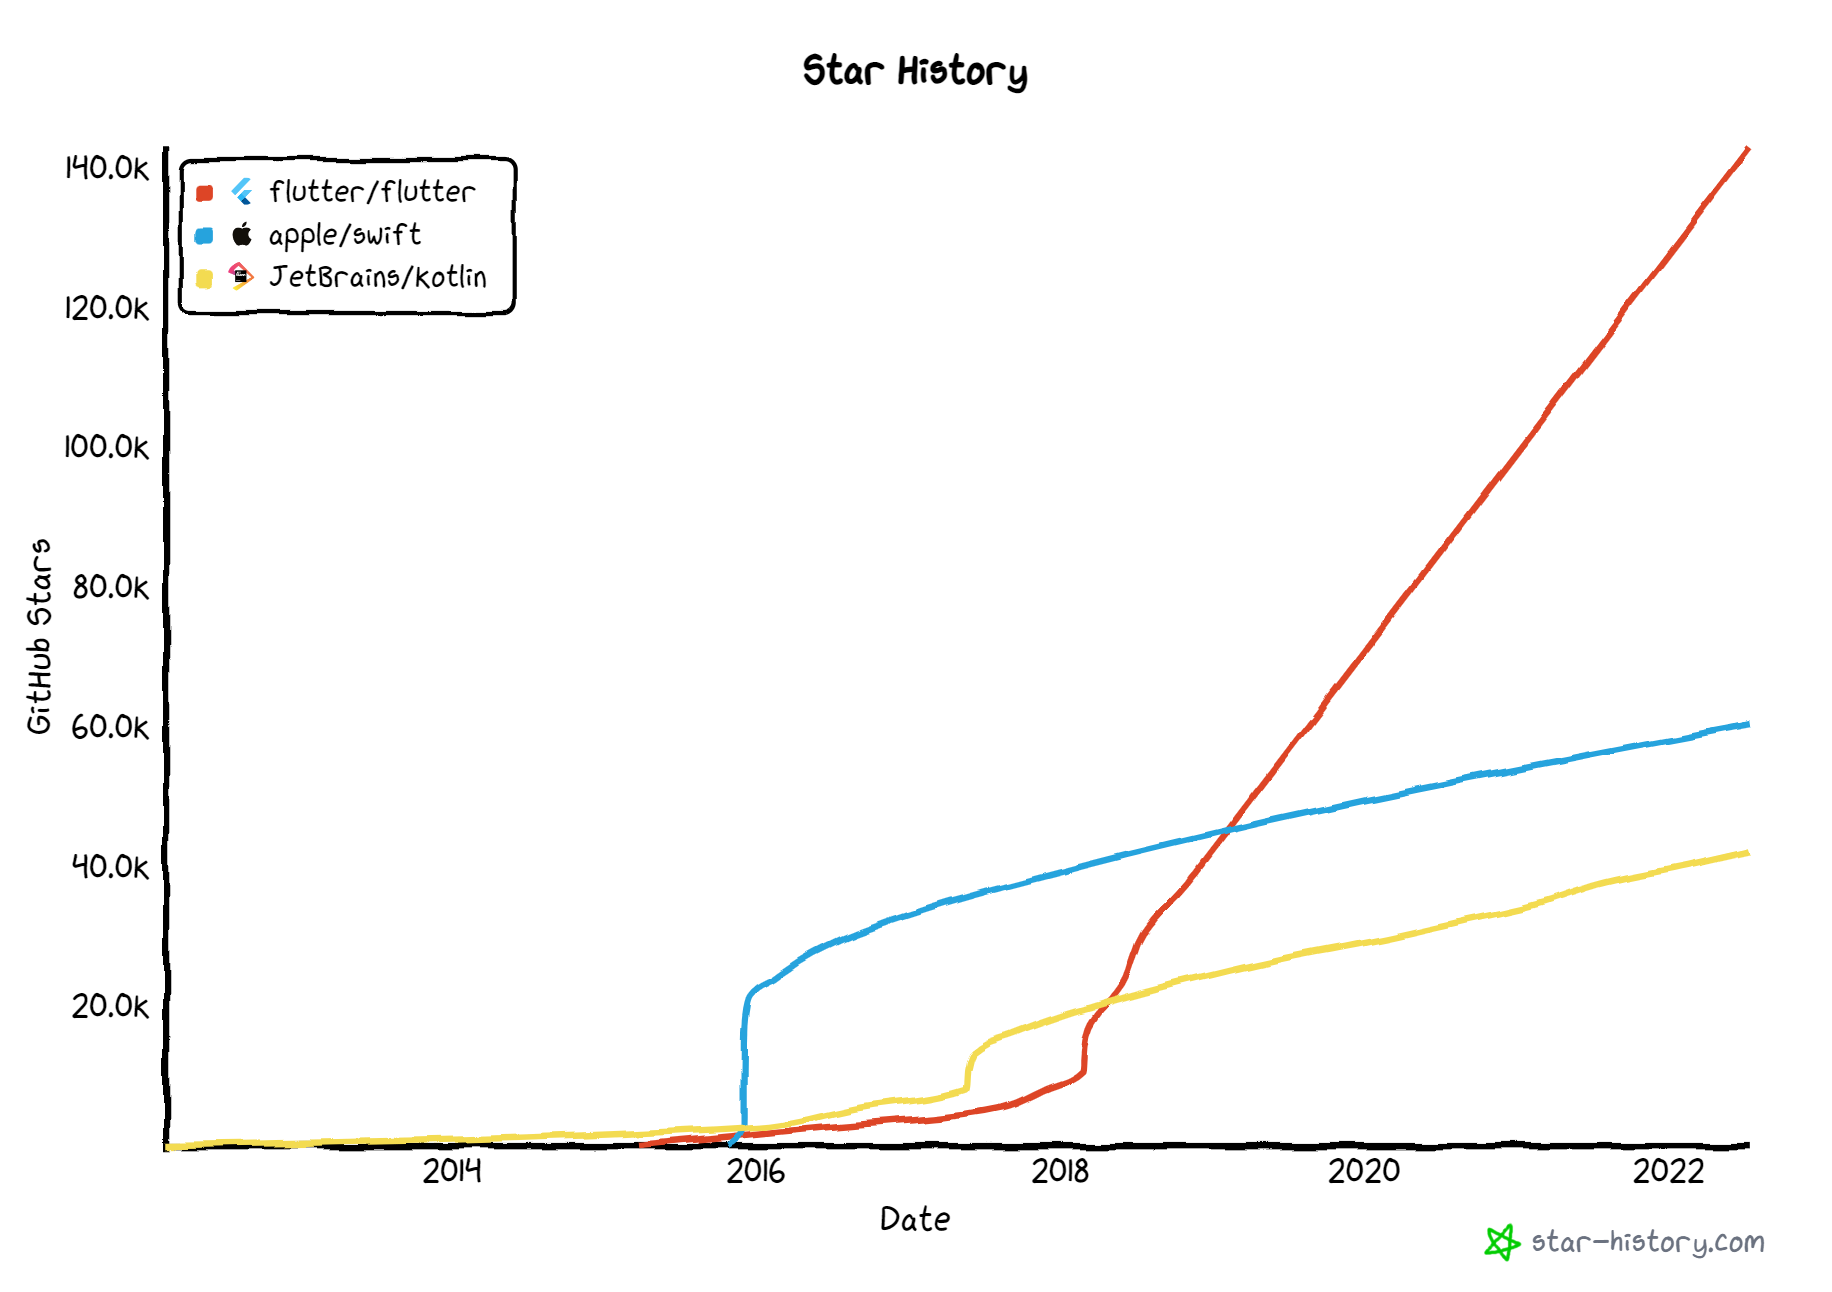
\includegraphics[height=8.5cm,keepaspectratio]{images/star-history_programming languages.png} 
  \caption[Zeitlicher Verlauf von Stars der Github-Repositories von Swift, Kotlin und Flutter]{Zeitlicher Verlauf von Stars der Github-Repositories von Swift, Kotlin und Flutter\protect\footnotemark }
  \label{fig:star_history}
\end{figure}
\footnotetext{\url{https://star-history.com/\#flutter/flutter\&JetBrains/kotlin\&apple/swift\&Date}}



Abbildung \ref{fig:star_history} zeigt ein, mit Hilfe der GitHub-API erstelltes, Diagramm. Darin wird die Anzahl der Stars der Swift, Kotlin und Flutter Repositories im zeitlichen Verlauf angezeigt. 
Besonders gut zu erkennen ist, wie stark das Interesse an Flutter ist. Nach der ersten Ankündigung 2018 und der darauf ersten veröffentlichten Version ist die Zahl der Stars innerhalb von 4 Jahren auf 140 000 angestiegen. Die Repositories für Swift und Kotlin haben im gleichen Zeitraum gerade einmal 20 000 Stars dazu erhalten. Zwar haben Swift und Flutter beide innerhalb des ersten Jahres nach ihrer Vorstellung etwa 30 000 Stars erhalten. Jedoch ist das Interesse an beiden nach einer anfänglichen Phase abgeflacht und verlaufen danach parallel zueinander.

\subsubsection{Stackoverflow}
Ein anderer Anhaltspunkt für die Größe einer Entwicklergemeinschaft ist die Anzahl der gestellten Fragen auf Stackoverflow. Stackoverflow bietet eine Plattform, um Fragen zu Entwicklungsproblemen zu stellen. Diese können von anderen Entwicklern beantwortet werden. So können generelle Ideen diskutiert und kleine Code-Stücke ausgetauscht werden. Stackoverflow ermöglicht es angemeldeten Nutzern, unter entsprechender Filterung, die Anzahl der gestellten Fragen für einen Suchbegriff zu bestimmen. Hierfür wurde die Anzahl der Fragen bezüglich Kotlin, Swift und Flutter innerhalb der letzten 2 Jahre bestimmt. Zusätzlich wurde auch noch die Anzahl der insgesamt gefundenen Fragen bestimmt. Dabei wurden eventuelle Überschneidungen mit anderen Programmiersprachen, sowie unbeantwortete Fragen herausgefiltert.

\begin{table}[ht]
\centering
\caption{Anzahl gefundener Fragen pro Programmiersprache}
\begin{tabular}{ |p{3.7cm}||>{\raggedleft\arraybackslash}p{5cm}|>{\raggedleft\arraybackslash} p{5cm}|}
 \hline
 \multicolumn{1}{|>{\centering\arraybackslash}p{3.7cm}||}{Programmiersprache} &
 \multicolumn{1}{>{\centering\arraybackslash}p{5cm}|}{Anzahl gefundener Fragen der letzten 2 Jahre} &
 \multicolumn{1}{>{\centering\arraybackslash}p{5cm}|}{insgesamt gefundene Fragen}\\
 \hline
 Kotlin &  105 082 Fragen\tablefootnote{Filter: [kotlin] or [android][kotlin] or [android]-[flutter]-[java] lastactive:2y.. is:question answers:1..} & 920 585 Fragen\\
  \hline
 Swift  & 71 749 Fragen\tablefootnote{Filter: [swift] or [ios][swift] or [ios]-[flutter]-[objectivc] lastactive:2y.. is:question answers:1..} & 670 697 Fragen\\
  \hline
 Flutter & 77 568 Fragen\tablefootnote{Filter:[flutter] or [dart] -[ubuntu] lastactive:2y.. is:question answers:1..} & 115 533 Fragen\\
 \hline
\end{tabular}
\label{tab:evaluations_questions_stackoverflow}
\end{table}

Tabelle \ref{tab:evaluations_questions_stackoverflow} zeigt die ermittelten Werte. Flutter hat hierbei in den letzten zwei Jahren eine ähnlich aktive Community wie Kotlin und Apple. Hier muss jedoch bedacht werden, dass Fragen, die bereits vor dem Untersuchungszeitraum gestellt wurden, innerhalb dieses Zeitraumes nicht erneut gestellt wurden. Deswegen wurde die insgesamte Anzahl der Fragen ebenfalls betrachtet. Hierbei ist die Anzahl sowohl bei Kotlin als auch Swift deutlich höher. Jedoch wurde diese beiden Technologien früher als Flutter veröffentlicht.
Für Flutter zeigt sich, dass in den letzten 2 Jahren eine ähnlich große Community wie für Kotlin und Swift existiert.

\subsubsection{Dokumentation}
Ein weiterer Faktor ist die Dokumentation. Sowohl Flutter als auch Kotlin und Swift veröffentlichen eine umfangreiche und von den Entwicklern dauerhaft aktualisierte Dokumentationsseite. Jedoch besitzt Flutter im Gegensatz zu Android und iOS einen offiziellen zentralen Ort\footnote{\url{https://pub.dev/}}, um nach externen Packages zu suchen. Hier sind neben den offiziellen von Flutter veröffentlichten Repositories, auch von der Community entwickelte Packages verlinkt. In der Summe können hier bereits über 27000 Erweiterungen gefunden werden\footnote{\url{https://pub.dev/packages?q=}}. Neben einem Punktesystem, dass diese bezüglich der Einhaltung von Richtlinien bewertet, werden außerdem die unterstützten Plattformen angezeigt. Zwar gibt es auch Bemühungen ein solches Verzeichnis für Kotlin und Swift einzuführen, jedoch sind diese nicht offiziell von den Entwicklerfirma betrieben und oft nicht vollständig.

Neben der Dokumentation für die Programmiersprache, existieren weitere Dokumentationen für die verschiedenen Entwicklungsansätze. Dabei sind sowohl für den cross-kompilierten als auch für den nativen Ansatz eine umfangreiche Dokumentation verfügbar, da sie der Standardentwicklungsmethode der Programmiersprache folgen. Für den gewählten hybriden Ansatz konnte anhand von Anleitungen und Dokumentation der Programmiersprache eine ausreichende Basis gefunden werden. Lediglich der gemischte Ansatz verfügte über keine Dokumentation. Zwar existiert gute Dokumentation für die gewählten Grundlagen und die Web-Implementierung, jedoch ist nur wenig Dokumentation für den genauen Ansatz und die Kombination der Technologien vorhanden. Dies wird jedoch durch die Art der Implementierung bedingt, da viele verschiedene gemischte Implementierungen möglich sind. Diese besitzen dabei oft eher einen experimentellen Charakter.

Zusammenfassend wird ersichtlich, dass bei einer normalen Nutzung der Programmiersprache beziehungsweise des Frameworks, eine umfangreiche Dokumentation gefunden werden kann. Je mehr sich jedoch von der normalen Nutzung entfernt wird, desto geringer wird die Dichte an verfügbaren Materialien. 

\subsubsection{Entwickler}
Ein letzter Faktor, der zu dieser Kategorie analysiert werden soll, ist die Anzahl der verfügbaren Entwickler. Eine Befragung \cite{statist_used_programming_languages} von 71 547 Entwicklern der Firma Stackoverflow zeigt, dass etwa 9\% Kotlin, 7\% Dart und 5\% Swift beherrschen.
Bei den Programmiersprachen der Webtechnologien, gaben 65\% an, JavaScript zu kennen und 55\% können mit HTML beziehungsweise CSS entwickeln. Diese Zahlen lassen den Schluss zu, dass die Ansätze mit einem hohen Anteil an Web-Technologie einen Vorteil haben, da es mehr Entwickler für diese Ansätze gibt. Jedoch wird auch bei diesen Ansätzen mindestens ein Entwickler benötigt, der sich mit den einzelnen Plattformen genauer auskennt. 
Ansonsten ist die Entwicklung eigener plattformspezifischer Funktionalität nicht möglich.

\section{Entwicklungsdauer}
Ein weiteres wichtiges Kriterium bei der Wahl des Ansatzes ist die Entwicklungsdauer, da diese sich auf die Kosten der entwickelten Multi-Plattform-Anwendung auswirkt. Außerdem sollen Applikationen möglichst schnell entwickelt und an den Nutzer verteilt werden können. Daher soll zusätzlich die Zeit betrachtet werden, bis die Applikation beziehungsweise ein Update bei den Nutzern verfügbar ist.

\subsubsection{Programmieraufwand}
Die genaue Entwicklungsdauer ist stark von der Erfahrung der Entwickler und eventuell auftretenden Problemen während der Implementierung abhängig. Folglich ist ein Zeitvergleich hier nicht sinnvoll. Stattdessen soll die Anzahl der geschriebenen Programmzeilen / Lines of Code (LOC) betrachtet werden.
Dafür wurden die einzelnen Daten mit Hilfe des Statistics\footnote{\url{https://plugins.jetbrains.com/plugin/4509-statistic}} Plug-In von JetBrains gesammelt.
Bei den beiden Implementierungen mit Web-Anteil wurde außerdem der notwendige Teil der Web-Implementierung mit angegeben. 
Die gesammelten Daten wurden in drei Teile aufgeteilt: Konfiguration, Benutzeroberfläche und Logik. 
Bei den Implementierungen, welche Flutter benutzen, ist der UI- und Logikcode zusammengefasst, da dies bei Flutter nicht unterschieden werden kann.
Als weiterer Parameter wurde der benötigte Code untersucht, um eine Liste an Objekten anzuzeigen.
Dabei wurde automatisch generierter Code nicht gezählt, sondern nur der tatsächlich geschriebene.

\begin{table}[ht]
\centering
\caption[Programmlänge der verschiedenen Implementierungen in LOC]{Programmlänge der verschiedenen Implementierungen in LOC}
\begin{tabular}{ |p{3.5cm}||>{\raggedleft\arraybackslash}p{2.5cm}|
>{\raggedleft\arraybackslash}p{2.5cm}|
>{\raggedleft\arraybackslash}p{3.5cm}|
>{\raggedleft\arraybackslash}p{2.5cm}|}
 \hline
 \multicolumn{1}{|>{\centering\arraybackslash}p{3.5cm}||}{} &
 \multicolumn{1}{>{\centering\arraybackslash}p{2.5cm}|}{native\break Applikation}  &
 \multicolumn{1}{>{\centering\arraybackslash}p{2.5cm}|}{hybride\newline Applikation} &
 \multicolumn{1}{>{\centering\arraybackslash}p{3.5cm}|}{cross-kompilierte Applikation} &
 \multicolumn{1}{>{\centering\arraybackslash}p{2.5cm}|}{gemischte Applikation} \\
 \hline
 Gesamte\break Anwendung      & 3138 & 215(App) + 2814(Web) & 2100 & 2391(App) + 1533(Web) \\ \hline
 Konfigurationscode           & 229  & 30 + 357             & 32   & 42 + 268              \\ \hline
 Oberflächencode              & 1958 & 86 + 1768            &\multirow{2}{*}{2068}  &\multirow{2}{*}{2349 + 1265} \\
  \cline{1-3}
 Funktionalität \& Logik  & 951& 99 + 689& &\\
  \hline
 Beispiel: Liste an Gegenständen & 178  & 71(Web)              & 65   & 65(App)               \\ \hline
\end{tabular}
\label{tab:lines_of_code}
\end{table}

Die in Tabelle \ref{tab:lines_of_code} zu sehende Aufschlüsselung zeigt, dass Flutter insgesamt die wenigsten Zeilen Code benötigt. 
Dabei werden gerade einmal 32 Zeilen Code Konfiguration benötigt. 
Der Rest sind knapp 2000 Zeilen Code mit Benutzeroberfläche und Logik.
Den höchsten Programmieraufwand in diesem Vergleich benötigt der gemischte Ansatz. Er kommt insgesamt auf circa 4000 Zeilen Code und benötigt damit rund doppelt so viel wie die Flutter Implementierung. 
Die native und die hybride Implementierung haben in etwa gleich viele Zeilen Code und liegen mit rund 3000 Zeilen Code zwischen den zwei anderen Implementierungen.

Bei dem zusätzlich betrachteten Beispiel, einer dynamischen Liste für Gegenstände ohne feste Länge, ist die Flutter Implementierung ebenfalls die Kürzeste. Dabei werden gerade einmal 65 Zeilen Code benötigt, wovon 55 Zeilen auf die Anzeige eines Gegenstandes und gerade einmal 10 Zeilen Code auf die Liste entfallen. Ähnlich verhält sich dies bei der Implementierung mit einer Webseite. Einzig die native Kotlin Applikation hat hierbei einen erhöhten Aufwand. Dabei fallen 75 Zeilen für das Design und weitere 83 Zeilen für die Steuerung der Liste an. Ein Großteil davon ist der Adapter, der benötigt wird, um die Liste zu steuern. 

Ebenfalls muss beachtet werden, wie viele Implementierungen je Ansatz benötigt werden. So ist bei dem gemischten und dem cross-kompilierten Ansatz lediglich die eine vorgestellte Implementierung nötig. Bei dem nativen Ansatz muss jedoch pro unterstützte Plattform eine eigenständige Implementierung erstellt werden. Bei der hybriden Applikation, wie sie in dieser Arbeit umgesetzt wurde, ist zwar die umgebende Applikation ebenfalls für jede Plattform zu implementieren, jedoch hat die Implementierung einen deutlich geringeren Umfang, da der Teil der Web-Anwendung lediglich einmalig zu programmieren ist.  

Es wurde gezeigt, dass eine cross-kompilierte Lösung mit Flutter deutlich weniger Zeilen Code als die anderen Implementierungen benötigt.
Sollte jedoch bereits eine Web-Anwendung existieren, reduziert sich der Implementierungsaufwand der hybriden Applikation auf knapp 200 Zeilen Code und die gemischte Implementierung halbiert sich in etwa. Dadurch können diese beiden Implementierungen dann ebenfalls eine gute Alternative zu den anderen Ansätzen darstellen. Muss diese jedoch erst erstellt werden, ist gerade der gemischte Ansatz mit einem erhöhten Aufwand verbunden. Außerdem wurde festgestellt, dass mit mehr unterstützten Plattformen der native Ansatz sich im Aufwand multipliziert.

\subsubsection{Zeit bis zur Veröffentlichung der App und von Updates }
Die Entwicklungsdauer wirkt sich auch auf die Dauer bis zur Veröffentlichung einer ersten Version aus.
Je früher eine Anwendung veröffentlicht werden kann, desto früher können Kunden die Applikation nutzen und bei einer kommerziellen Nutzung folglich auch Umsatz produzieren.

Hier haben die gemischte und die hybride Implementierung den Vorteil, dass bei einer bereits bestehenden Webseite, die Zeit bis zur Veröffentlichung einer ersten Version sehr gering ist, da bereits wenige Zeilen Code die Webseite in der App anzeigen. Zu einem späteren Zeitpunkt können mehr Funktionalitäten und Optimierungen in kommende Versionen hinzugefügt werden. Wenn jedoch keine Webseite besteht, ist die anfängliche Dauer vergleichbar, beziehungsweise etwas höher als bei der cross-kompilierten Implementierung. Lediglich die native Implementierung benötigt durch das Erstellen der verschiedenen Plattform-Applikation deutlich mehr Zeit. Dies kann zwar durch zusätzliche Entwickler begrenzt werden, jedoch steigen dadurch die Entwicklungskosten.

Bei der Veröffentlichung von Updates zeigt sich ein weiterer Vorteil der Nutzung einer Webseite innerhalb einer Applikation. So können Updates auf der Webseite sofort verteilt werden und müssen nicht über den App-Store der verschiedenen Geräte verteilt werden. Die Veröffentlichung von Apps oder deren Updates kann dabei zwischen einem Tag und einer Woche dauern\footnote{\url{https://developer.apple.com/app-store/review/}} \footnote{\url{https://qr.ae/pvu0ud}}. Diese Zeit wird dafür bei jeder Änderung an der App bei allen vier Ansätzen benötigt.

\section{Benutzeroberfläche}
Die Bewertung einer Benutzeroberfläche ist stark von der persönlichen Präferenz abhängig. So empfinden Nutzer unterschiedlich, was eine gute Benutzeroberfläche ausmacht. Folglich soll in dieser Arbeit nicht auf das genaue Aussehen eingegangen werden, sondern auf einige allgemeine Eigenschaften der unterschiedlichen Benutzeroberflächen.

\subsubsection{Aussehen der Applikationen}
Grundsätzlich ist das Aussehen der Applikation vor allem davon abhängig, wie viel Zeit investiert wird, um ein angestrebtes Design zu erhalten. Um die unterschiedlichen Startseiten vergleichbar zu halten, wurde deswegen eine Maximalzeit für die Verwirklichung des Designs festgelegt. Diese Maximalzeit orientiert sich an der benötigten Entwicklungszeit der entsprechenden Web-Ansicht. Dafür wurde außer für den Schriftzug mit Farbverlauf keine externen Design-Pakete oder Erweiterungen benutzt. Eine zusätzliche Anforderung war dabei, dass die Seiten für unterschiedliche Bildschirmgrößen benutzbar sein müssen.

\begin{figure}[ht]
  \centering
  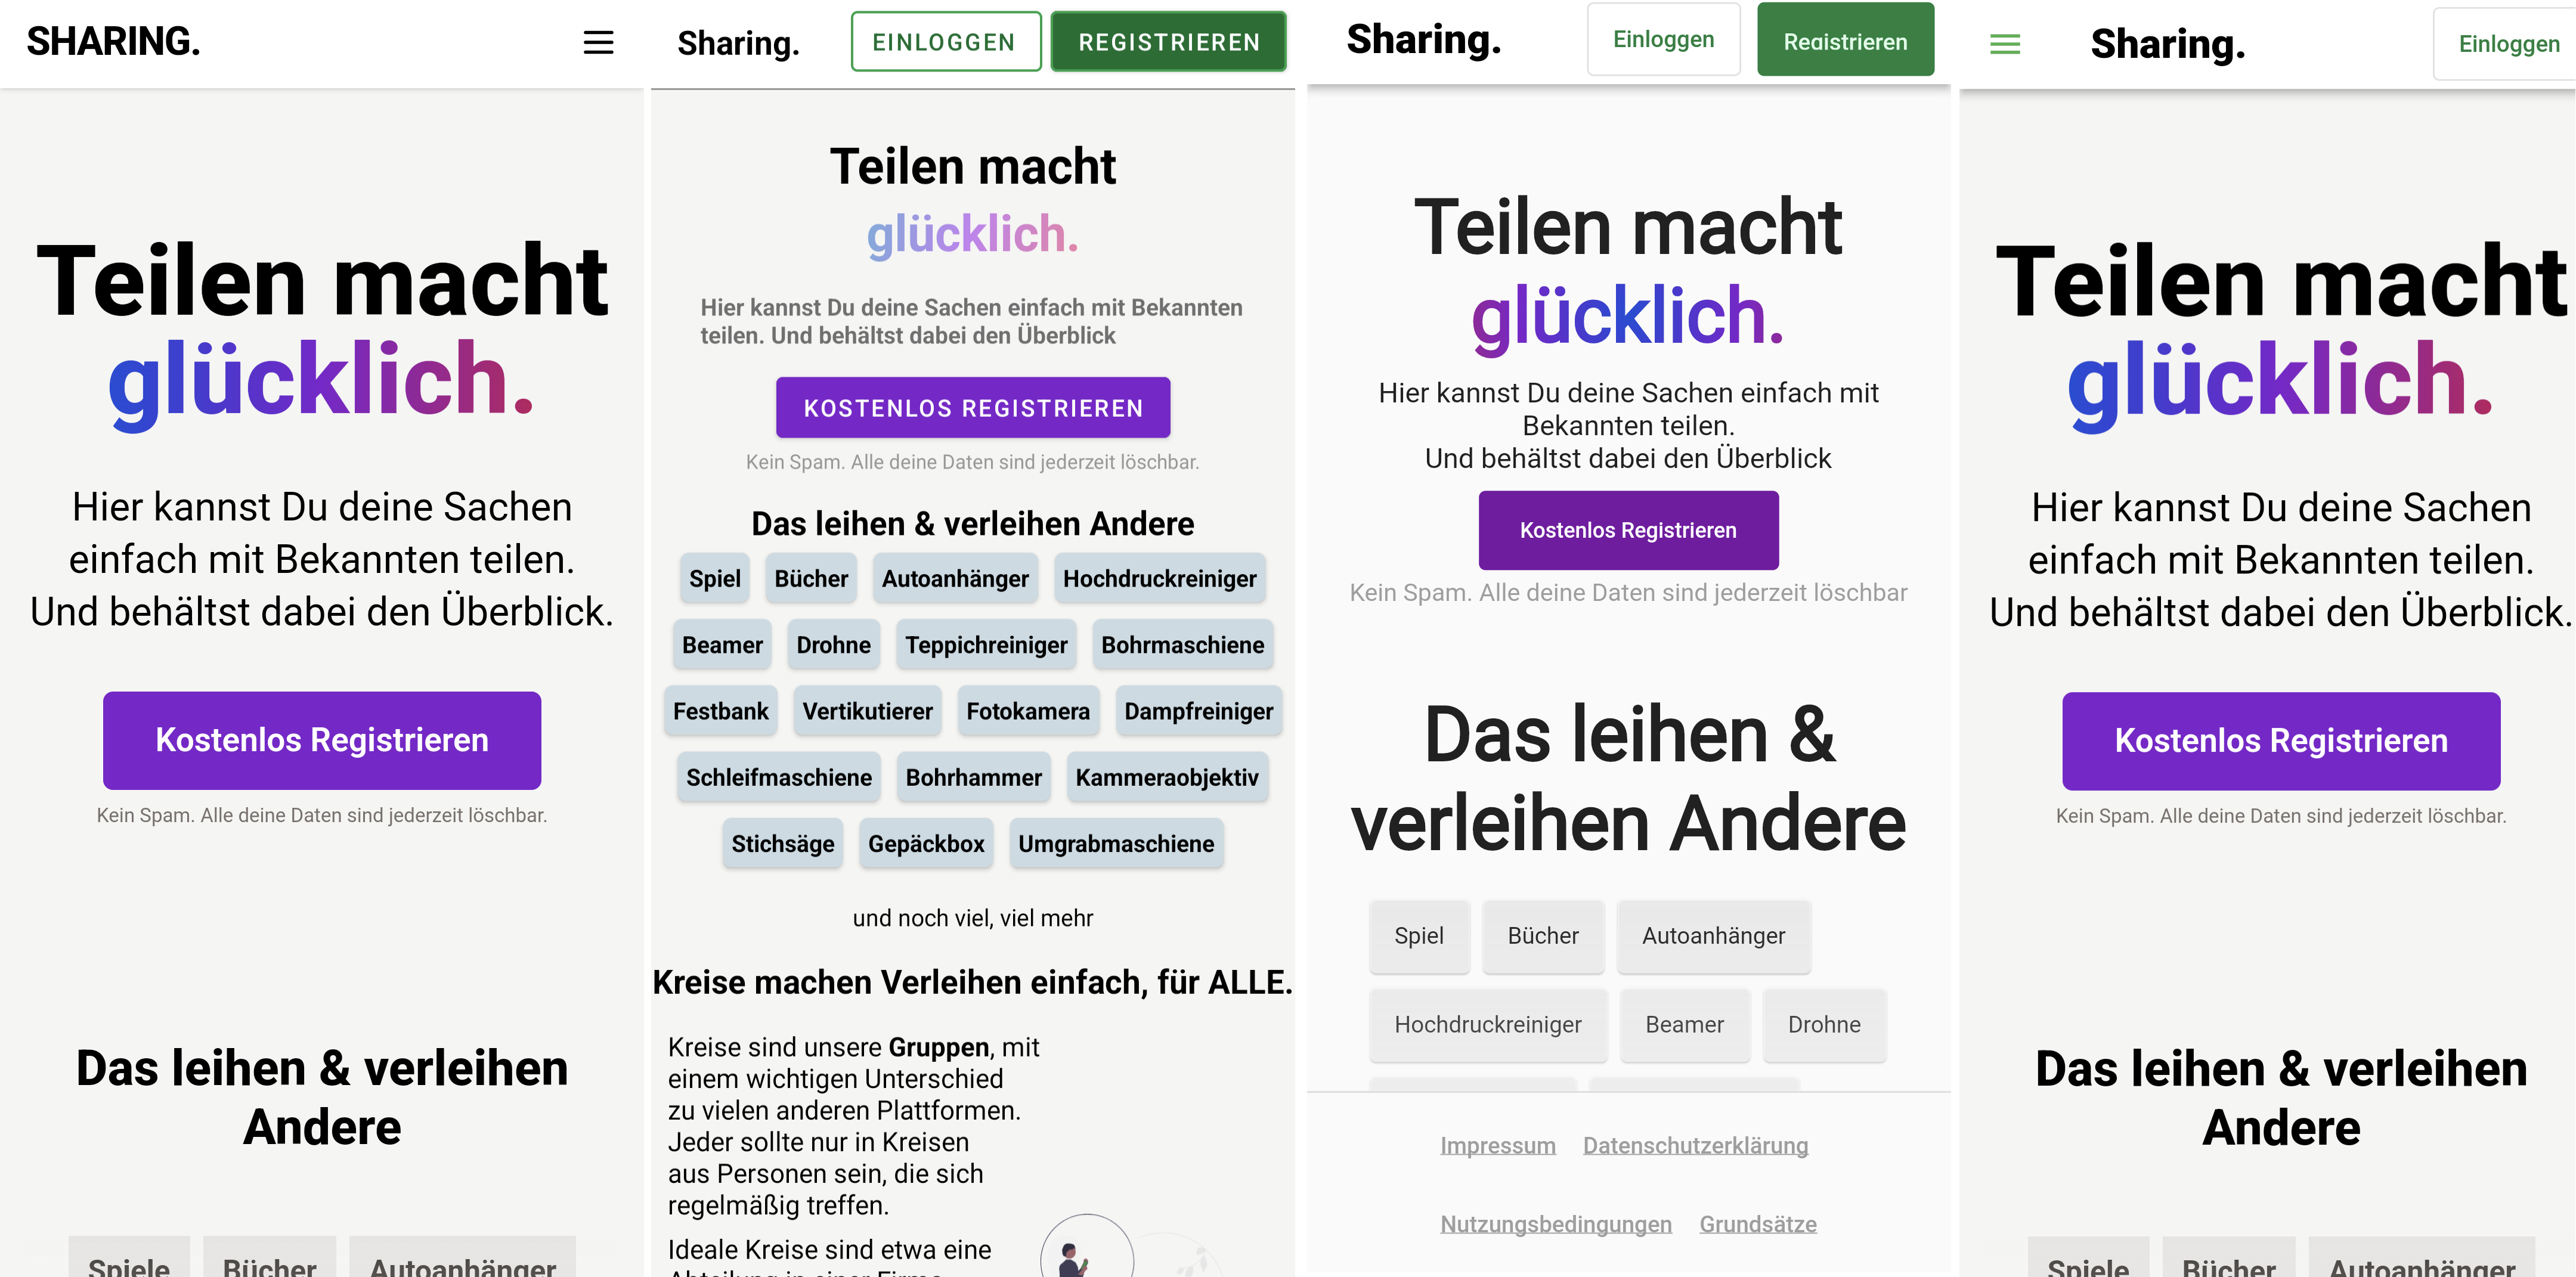
\includegraphics[height=7cm,keepaspectratio]{images/Startbildschirm_vergleich.png} 
  \caption[Vergleich des Startbildschirms der Implementierungen]{Vergleich des Startbildschirms der Implementierungen.\break Von links nach rechts: Hybride-Applikation, native Kotlin Applikation, Flutter Cross-Plattform-Applikation, gemischte Flutter Applikation}
  \label{fig:startscreen}
\end{figure}

In Abbildung \ref{fig:startscreen} sind die Startbildschirme der verschiedenen Anwendungen zu sehen. Dabei zeigen das erste und letzte Bild die Startseite der Webseite. Die zwei mittleren Bilder zeigen die im App-Code definierten Seiten. Grundsätzlich kann dabei festgestellt werden, dass die Seiten ähnlich aussehen, lediglich die Größe des Textes unterscheidet sich zwischen den Versionen stark.

Bei dem ersten Bildschirm, welcher von der hybriden Applikation stammt, musste am Design der Applikation nicht viel angepasst werden, da die Webseite bereits für die Nutzung an einem mobilen Endgerät angepasst war. Jedoch fallen bei der Benutzung Unterschiede zur nativen beziehungsweise Flutter Entwicklung auf. 
Um dies zu verdeutlichen zeigt Abbildung \ref{fig:sidemenu} die Seitenmenüanzeigen der Flutter-Anwendung (links) und der Webimplementierung (rechts). Hierbei ist klar zu erkennen, dass die Web-Implementierung für PC-Nutzer ausgelegt ist, da das Menü für eine Anklick-Bedienung optimiert ist. 
Im Gegensatz dazu kann das Seitenmenü bei der Flutter Implementierung über eine Wischgeste geöffnet werden und wird dabei über den gesamten Gerätebildschirm angezeigt, während bei der Webseite das Menü nur innerhalb des Web-Containers angezeigt wird. Dadurch erhält der Nutzer in der Flutter Applikation den Eindruck, dass sich das Menü über die restliche UI legt. 
\begin{figure}[ht]
  \centering
  \includegraphics[height=7cm,keepaspectratio]{images/Seitenmenü_vergleich.png} 
  \caption[Vergleich des Seitenmenüs der nativen und hybriden Applikation]{Vergleich des Seitenmenüs bei nativer Implementierung (links) und JavaScript Implementierung (rechts)}
  \label{fig:sidemenu}
\end{figure}

Während auf der Webseite eine umfangreiche Design-Implementierung genutzt wurde, um das Aussehen der Anwendung zu verändern, wurden bei der nativen Kotlin und den Flutter Implementierungen lediglich die Farben und Textgrößen angepasst. Dies wurde gemacht, um einen Eindruck für die Standardkonfiguration des Designs der verschiedenen Implementierungen vergleichen zu können. Bei der Flutter Implementierung wirken die Elemente im Gegensatz zur nativen Implementierung moderner und besser an ein Smartphone angepasst. Dies wird deutlich, wenn die Login-Seite verglichen wird.

\begin{figure}[ht]
  \centering
  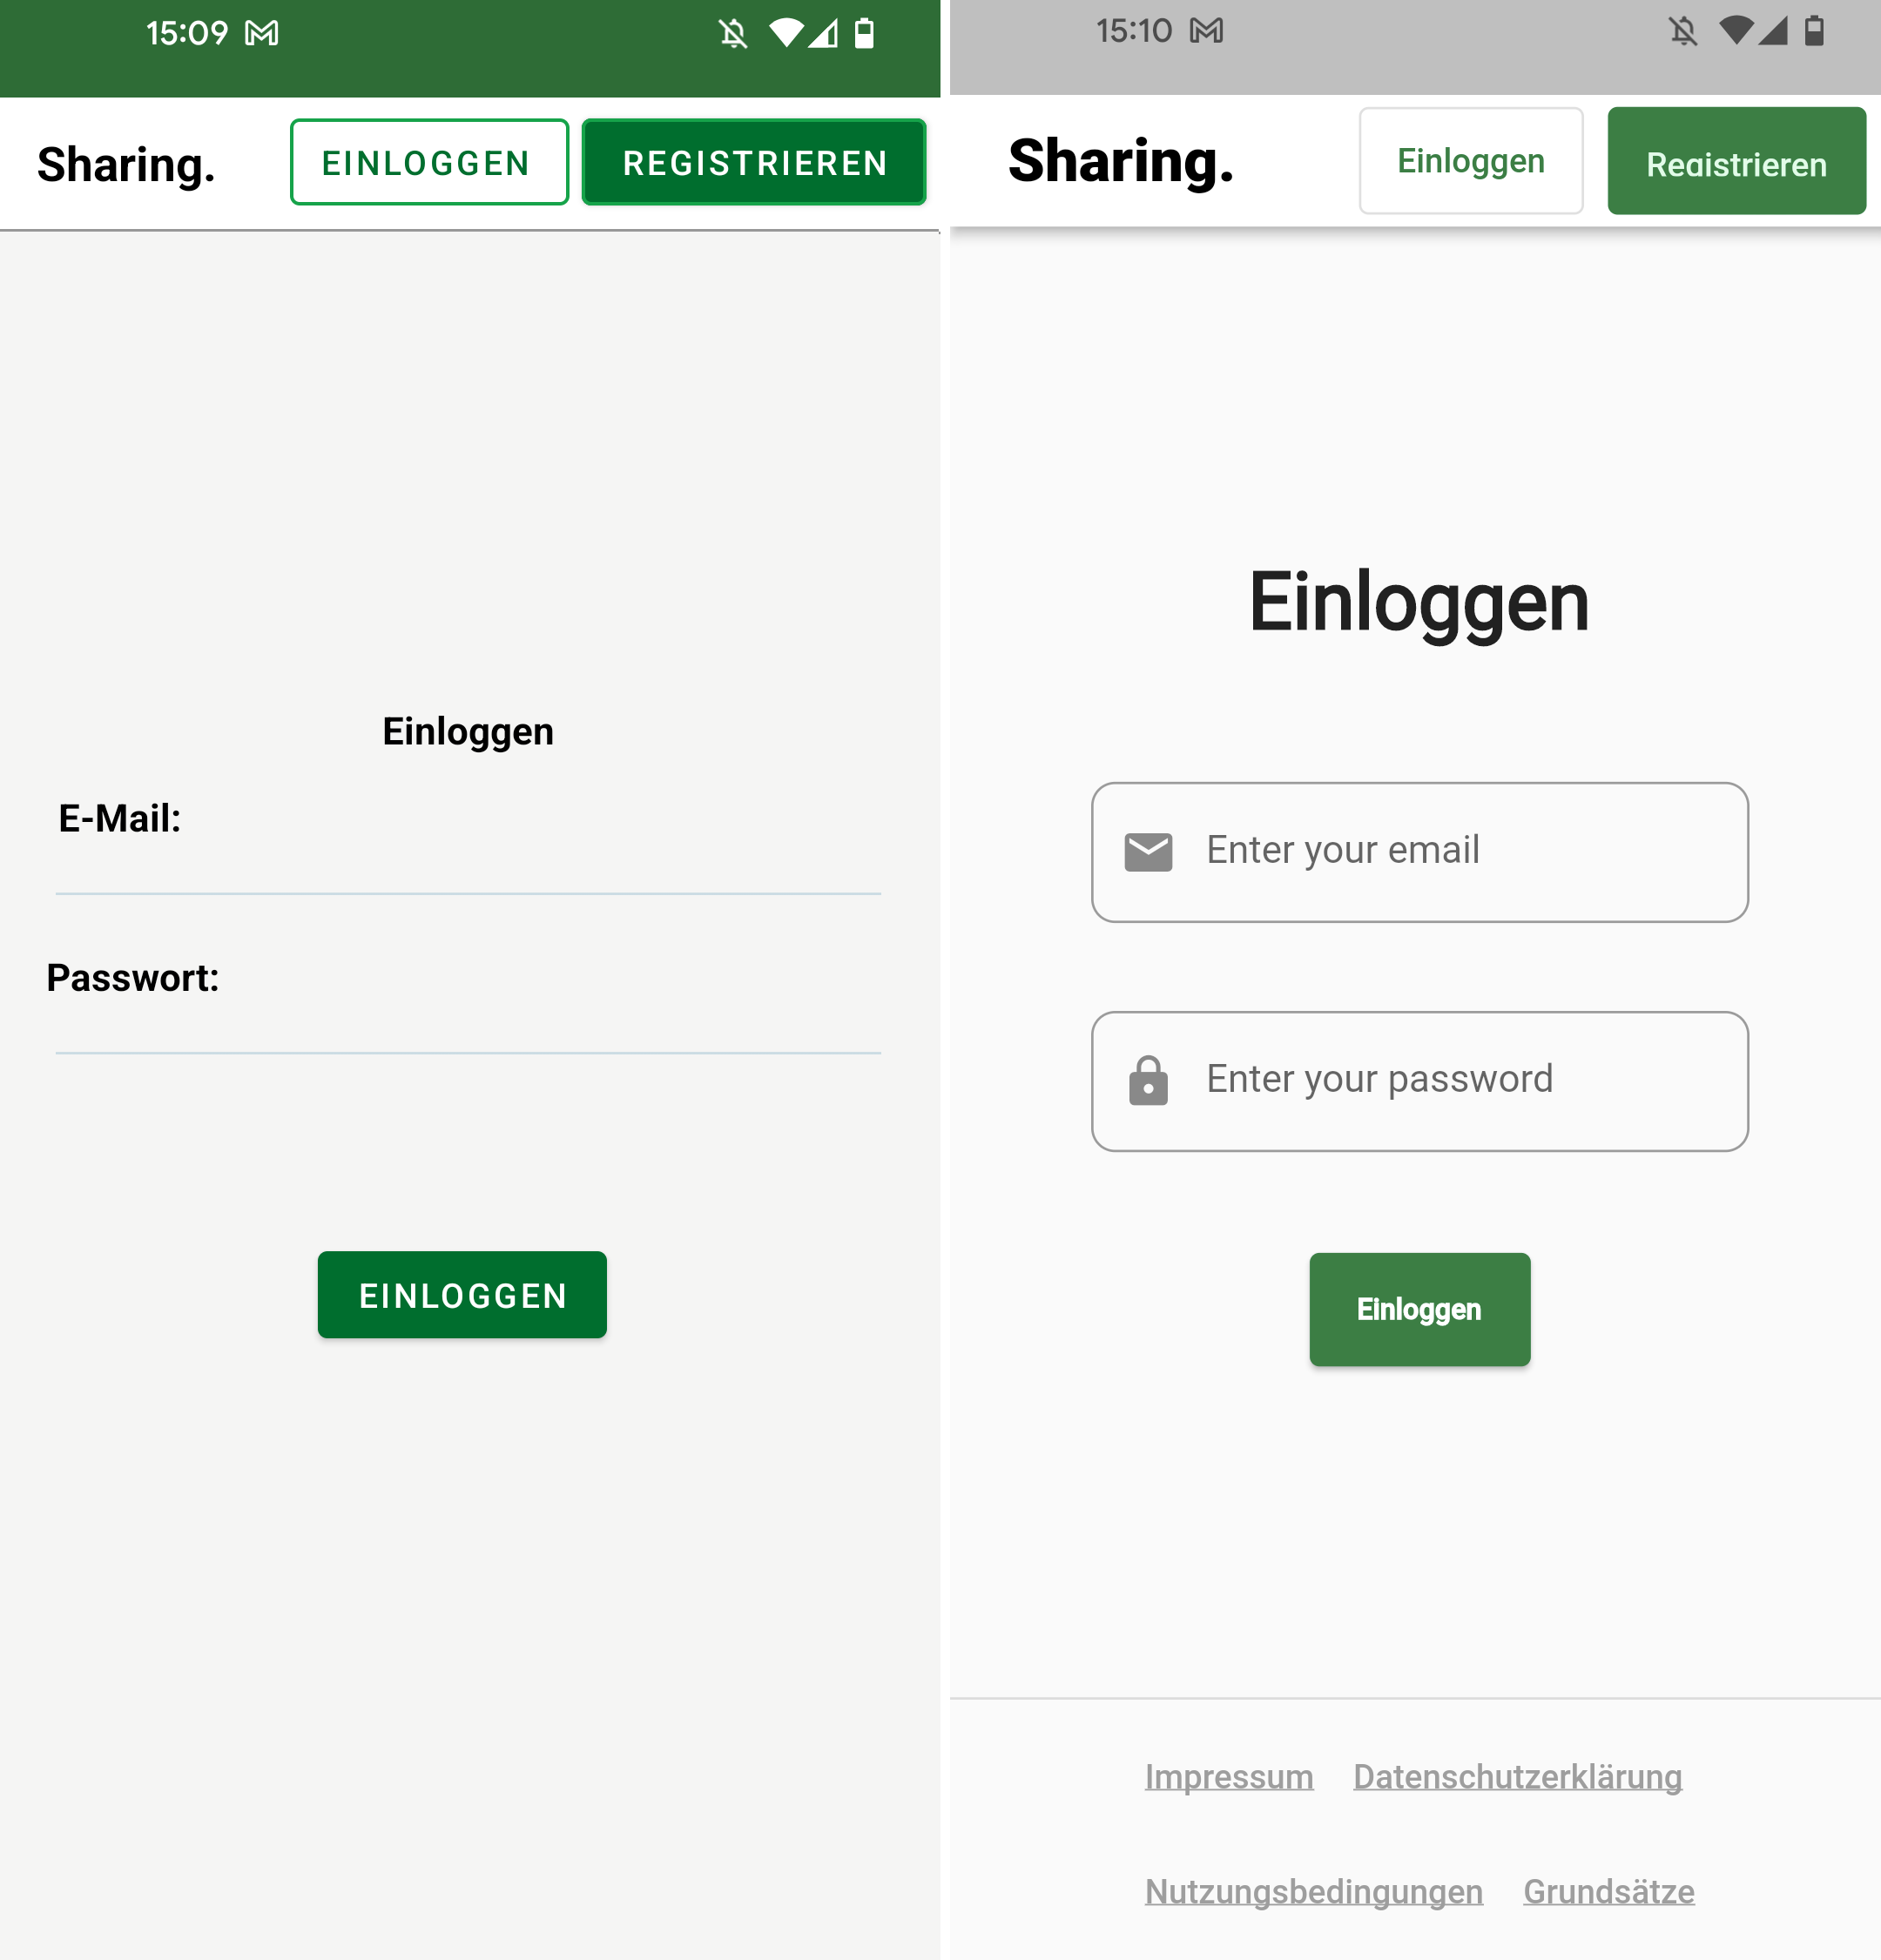
\includegraphics[height=7cm,keepaspectratio]{images/Login_vergleich.png} 
  \caption[Vergleich des Login-Bildschirms von Kotlin und Flutter Implementierung.]{Vergleich des Login-Bildschirms von Kotlin (links) und Flutter (rechts) Implementierung}
  \label{fig:loginscreen}
\end{figure}

In Abbildung \ref{fig:loginscreen} sind die Login-Seiten der nativen und des cross-kompilierten Ansatzes zu sehen. Dabei zeichnet sich Flutter durch ein besseres \grqq{}Out-of-the-Box\grqq{} Design-Paket aus. So ist das Input Feld bei der Kotlin Implementierung lediglich durch einen Strich definiert und kann dadurch für einen Nutzer schwer zu finden sein. Flutter hingegen hat als Standardinputfeld ein umrahmtes Feld, dass durch Hinzufügen von Werten auf vordefinierten Attributen beliebig und einfach im Style angepasst werden kann. Bei der nativen Implementierung ist dies zwar ebenfalls möglich, allerdings entsteht dadurch zusätzlicher Aufwand.

Während der Entwicklung konnte festgestellt werden, dass mit genügend Zeit und den richtigen Erweiterungen, jede Benutzeroberfläche in das gewünschte Format zu bringen ist. Vor allem bei der Unterstützung unterschiedlicher Bildschirmgrößen benötigte jedoch die native Anwendung umfangreiche Anpassungen, während dies bei den anderen Ansätzen deutlich unkomplizierter zu erreichen war. Flutter unterstütze die Verwirklichung einer gutaussehenden Benutzeroberfläche insofern, dass die Standardkonfiguration Googles Design-Paket Material3\footnote{\url{https://m3.material.io/}} nutzt.

\subsubsection{Konsistenz über Plattformen hinweg}
Ein weiteres Ziel bei der Entwicklung der Benutzeroberfläche ist die Konsistenz über Plattformen hinweg.
Dabei soll der Nutzer keinen Unterschied bemerken, wenn er von einer Plattform zur anderen wechselt. 
Das Risiko solcher Inkonsistenzen ist bei unterschiedlichen Implementierungen für die einzelnen Plattformen höher, als wenn eine einzelne Code-Basis verwendet werden kann.

Dementsprechend haben Implementierungen, die für mehrere Plattformen wieder verwendet werden können, einen positiven Einfluss auf die Konsistenz.
Auf die in dieser Arbeit vorgestellten Implementierungen bezogen, bedeutet dies, dass die reine native Implementierung eine höhere Gefahr von Inkonsistenz besitzt als die hybride, gemischte oder cross-kompilierte Implementierung.
Dabei ist zu erwähnen, dass auch die nativen Applikationen einen hohen Grad an Konsistenz erreichen können. Dies erfordert jedoch wieder einen höheren Aufwand und eine enge Zusammenarbeit der Entwickler während der Implementierung der verschiedenen Plattformen.

\section{Funktionalität}
Als abschließendes Kriterium wird die Funktionalität der einzelnen Ansätze betrachtet. Dabei soll neben der Plattformabdeckung, die Möglichkeiten zur Nutzung von Offlinefunktionalität und Plattformfunktionalität betrachtet werden.

\subsubsection{Plattformabdeckung}
Wie bereits erwähnt, sind nativ entwickelte Applikationen immer nur für eine Plattform verwendbar. Sie haben dementsprechend auch wenig wiederverwendbaren Code. Allerdings kann für jede Plattform eine native Applikation geschrieben werden und folglich können alle Plattformen abgedeckt werden.

Bei der hybriden Implementierung muss ebenfalls eine Applikation für jede Plattform geschrieben werden, jedoch kann der gleiche Web-Code auf den unterschiedlichen Plattformen verwendet werden. Grundsätzlich können auch bei diesem Ansatz alle Plattformen unterstützt werden, dabei müssen jedoch die Anforderungen der verschiedenen App-Stores beachtet werden. Denn wie bereits erwähnt, verlangt beispielsweise Apple, dass Apps den Großteil der Funktionalität intern abbilden. Eine Implementierung, wie sie hier vorgestellt wurde, würde wahrscheinlich abgelehnt werden.

Flutter bietet eine Unterstützung für alle aktuell verfügbaren mobilen Plattformen an. Außerdem arbeiten sie an einer Möglichkeit, Flutter auch auf Embedded-Geräten auszuführen\footnote{\url{https://flutter.dev/multi-platform/embedded}}.
Somit können alle Plattformen abgedeckt werden. Jedoch kann die Plattformunterstützung der eigenen Applikation durch genutzte Bibliotheken eingeschränkt werden. Beispielsweise war die, in dieser Arbeit vorgestellte, cross-kompilierte Implementierung lediglich mit fünf der sechs Plattformen kompatibel, da der genutzte GraphQL-Client keine Web-Version unterstützt.

Die gemischte Implementierung unterstützt noch weniger Plattformen. So konnte aufgrund des genutzten Web-Containers die Applikation lediglich auf Android und iOS genutzt werden.
Daher ist es eventuell sinnvoll, vor der Wahl eines Ansatzes auch benötigte Technologien zu recherchieren und die verfügbaren Bibliotheken zu analysieren, um derartige Probleme bereits vor dem Start der Implementierung zu identifizieren.


\subsubsection{Offlinefunktionalität}
Es gibt einige Fälle, in denen der Nutzer eine Applikation benutzen will, auch wenn er aktuell über keine aktive Internetverbindung verfügt. In diesem Fall benötigt die Applikation eine Offlinefunktionalität.

Wie in dieser Arbeit erwähnt, sind die Implementierungen die eine Webseite als Teil ihrer Implementierung haben offline stark eingeschränkt oder haben keine Funktionalität. Im Falle der gemischten Implementierung kann eine Offlinefunktionalität zumindest teilweise erreicht werden, indem bei einer fehlenden Internetverbindung durch Flutter implementierte Seiten angezeigt werden. Die native und cross-kompilierte Lösung haben hier den Vorteil, dass ihre Benutzeroberfläche unabhängig von einer aktiven Internetverbindung nutzbar ist. Zwar kommen die angezeigten Daten von einem Server, jedoch können diese lokal zwischengespeichert werden. Diese Lösung ist dabei sowohl für die native, cross-kompilierte und gemischte Implementierung möglich. 

Zu beachten ist, dass einige hybride Frameworks Daten und Benutzeroberfläche lokal auf dem Gerät speichern und dadurch eine offline Funktionalität möglich wäre. Allerdings verschwinden dadurch die Vorteile der Nutzung einer online Version, wie etwa die einfache Verteilung von Updates.

\subsubsection{Nutzung von Plattformfunktionalität}
Wie bei der Vorstellung der unterschiedlichen Implementierungen aufgezeigt wurde, kann mit der richtigen Implementierung die Nutzung der Plattformfunktionalität bei jeder der vier Implementierungen ermöglicht werden. Jedoch konnte aufgezeigt werden, dass die Nutzung mit unterschiedlichem Aufwand verbunden ist. So ist dies bei der nativen Implementierung am einfachsten umsetzbar. Auch der cross-kompilierte und der gemischte Ansatz können vollständig, wie in Kapitel 4.3.3 vorgestellt, auf die nativen Funktionen zugreifen. Ebenfalls kann der hybride Ansatz native Funktionalität nutzen, muss dafür jedoch eine JavaScript-Schnittstelle nutzen. Dies birgt Gefahren, die beachtet und abgeschätzt werden müssen (siehe Kapitel 4.2.2). Hier hat der gemischte Ansatz insofern den Vorteil gegenüber dem hybriden, dass die Web-Ansichten, die Plattformfunktionalität benötigen, durch Flutter-Seiten ersetzt werden können. Somit ist ein sicherer und einfacher Zugriff wie bei der cross-kompilierten Implementierung möglich.
